%% -*- coding: utf-8 -*-
\documentclass[12pt,pagesize,paper=landscape,paper=192mm:108mm]{scrbook} 
%1920x1080 1280x720
\areaset[current]{192mm}{108mm}
\usepackage{calc}
\usepackage[T2A]{fontenc}
\usepackage[utf8]{inputenc}
\usepackage[english,russian]{babel}
\usepackage{microtype}
\usepackage{misccorr}
\usepackage{cmap}
%\usepackage[unicode=true]{hyperref}
\usepackage{graphicx}
\usepackage{amssymb}
\usepackage{amsmath}
%\usepackage{srcltx}
\usepackage{textcomp}
\usepackage{xspace}
%научные символы и смайлики \smiley \frownie
\usepackage{wasysym}
\usepackage{ccicons}
\begin{document}
\begin{titlepage}
  \vspace*{-1em}
  \begin{center}
    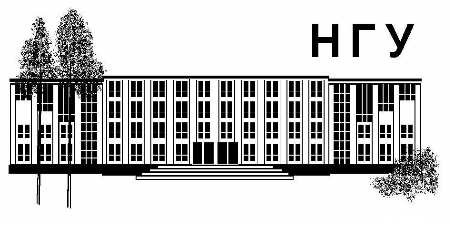
\includegraphics[width=0.23\textwidth]{../NSU-logo}

    Кафедра теоретической физики физического факультета НГУ
    \medskip

    \Large
    Профессор Черняк В.\,Л.
    \medskip

    \huge
    \textbf{Суперсимметрия в квантовой теории поля}
    \bigskip

    \Large
    Лекция № 22
    \vfill

    % \normalsize
    % \begin{minipage}{0.65\linewidth}
    % \end{minipage}
    \vfill

    \normalsize \ccbysa\hspace{0.5em}  Новосибирск 2013
  \end{center}
\end{titlepage}
\end{document}
